% Options for packages loaded elsewhere
\PassOptionsToPackage{unicode}{hyperref}
\PassOptionsToPackage{hyphens}{url}
%
\documentclass[
  ignorenonframetext,
]{beamer}
\usepackage{pgfpages}
\setbeamertemplate{caption}[numbered]
\setbeamertemplate{caption label separator}{: }
\setbeamercolor{caption name}{fg=normal text.fg}
\beamertemplatenavigationsymbolsempty
% Prevent slide breaks in the middle of a paragraph
\widowpenalties 1 10000
\raggedbottom
\setbeamertemplate{part page}{
  \centering
  \begin{beamercolorbox}[sep=16pt,center]{part title}
    \usebeamerfont{part title}\insertpart\par
  \end{beamercolorbox}
}
\setbeamertemplate{section page}{
  \centering
  \begin{beamercolorbox}[sep=12pt,center]{part title}
    \usebeamerfont{section title}\insertsection\par
  \end{beamercolorbox}
}
\setbeamertemplate{subsection page}{
  \centering
  \begin{beamercolorbox}[sep=8pt,center]{part title}
    \usebeamerfont{subsection title}\insertsubsection\par
  \end{beamercolorbox}
}
\AtBeginPart{
  \frame{\partpage}
}
\AtBeginSection{
  \ifbibliography
  \else
    \frame{\sectionpage}
  \fi
}
\AtBeginSubsection{
  \frame{\subsectionpage}
}
\usepackage{lmodern}
\usepackage{amssymb,amsmath}
\usepackage{ifxetex,ifluatex}
\ifnum 0\ifxetex 1\fi\ifluatex 1\fi=0 % if pdftex
  \usepackage[T1]{fontenc}
  \usepackage[utf8]{inputenc}
  \usepackage{textcomp} % provide euro and other symbols
\else % if luatex or xetex
  \usepackage{unicode-math}
  \defaultfontfeatures{Scale=MatchLowercase}
  \defaultfontfeatures[\rmfamily]{Ligatures=TeX,Scale=1}
\fi
\usetheme[]{Hannover}
\usecolortheme{dove}
\usefonttheme{structurebold}
% Use upquote if available, for straight quotes in verbatim environments
\IfFileExists{upquote.sty}{\usepackage{upquote}}{}
\IfFileExists{microtype.sty}{% use microtype if available
  \usepackage[]{microtype}
  \UseMicrotypeSet[protrusion]{basicmath} % disable protrusion for tt fonts
}{}
\makeatletter
\@ifundefined{KOMAClassName}{% if non-KOMA class
  \IfFileExists{parskip.sty}{%
    \usepackage{parskip}
  }{% else
    \setlength{\parindent}{0pt}
    \setlength{\parskip}{6pt plus 2pt minus 1pt}}
}{% if KOMA class
  \KOMAoptions{parskip=half}}
\makeatother
\usepackage{xcolor}
\IfFileExists{xurl.sty}{\usepackage{xurl}}{} % add URL line breaks if available
\IfFileExists{bookmark.sty}{\usepackage{bookmark}}{\usepackage{hyperref}}
\hypersetup{
  pdftitle={Session 9: Repeated Measures and Longitudinal Analysis I},
  pdfauthor={Levi Waldron},
  hidelinks,
  pdfcreator={LaTeX via pandoc}}
\urlstyle{same} % disable monospaced font for URLs
\newif\ifbibliography
\usepackage{color}
\usepackage{fancyvrb}
\newcommand{\VerbBar}{|}
\newcommand{\VERB}{\Verb[commandchars=\\\{\}]}
\DefineVerbatimEnvironment{Highlighting}{Verbatim}{commandchars=\\\{\}}
% Add ',fontsize=\small' for more characters per line
\usepackage{framed}
\definecolor{shadecolor}{RGB}{248,248,248}
\newenvironment{Shaded}{\begin{snugshade}}{\end{snugshade}}
\newcommand{\AlertTok}[1]{\textcolor[rgb]{0.94,0.16,0.16}{#1}}
\newcommand{\AnnotationTok}[1]{\textcolor[rgb]{0.56,0.35,0.01}{\textbf{\textit{#1}}}}
\newcommand{\AttributeTok}[1]{\textcolor[rgb]{0.77,0.63,0.00}{#1}}
\newcommand{\BaseNTok}[1]{\textcolor[rgb]{0.00,0.00,0.81}{#1}}
\newcommand{\BuiltInTok}[1]{#1}
\newcommand{\CharTok}[1]{\textcolor[rgb]{0.31,0.60,0.02}{#1}}
\newcommand{\CommentTok}[1]{\textcolor[rgb]{0.56,0.35,0.01}{\textit{#1}}}
\newcommand{\CommentVarTok}[1]{\textcolor[rgb]{0.56,0.35,0.01}{\textbf{\textit{#1}}}}
\newcommand{\ConstantTok}[1]{\textcolor[rgb]{0.00,0.00,0.00}{#1}}
\newcommand{\ControlFlowTok}[1]{\textcolor[rgb]{0.13,0.29,0.53}{\textbf{#1}}}
\newcommand{\DataTypeTok}[1]{\textcolor[rgb]{0.13,0.29,0.53}{#1}}
\newcommand{\DecValTok}[1]{\textcolor[rgb]{0.00,0.00,0.81}{#1}}
\newcommand{\DocumentationTok}[1]{\textcolor[rgb]{0.56,0.35,0.01}{\textbf{\textit{#1}}}}
\newcommand{\ErrorTok}[1]{\textcolor[rgb]{0.64,0.00,0.00}{\textbf{#1}}}
\newcommand{\ExtensionTok}[1]{#1}
\newcommand{\FloatTok}[1]{\textcolor[rgb]{0.00,0.00,0.81}{#1}}
\newcommand{\FunctionTok}[1]{\textcolor[rgb]{0.00,0.00,0.00}{#1}}
\newcommand{\ImportTok}[1]{#1}
\newcommand{\InformationTok}[1]{\textcolor[rgb]{0.56,0.35,0.01}{\textbf{\textit{#1}}}}
\newcommand{\KeywordTok}[1]{\textcolor[rgb]{0.13,0.29,0.53}{\textbf{#1}}}
\newcommand{\NormalTok}[1]{#1}
\newcommand{\OperatorTok}[1]{\textcolor[rgb]{0.81,0.36,0.00}{\textbf{#1}}}
\newcommand{\OtherTok}[1]{\textcolor[rgb]{0.56,0.35,0.01}{#1}}
\newcommand{\PreprocessorTok}[1]{\textcolor[rgb]{0.56,0.35,0.01}{\textit{#1}}}
\newcommand{\RegionMarkerTok}[1]{#1}
\newcommand{\SpecialCharTok}[1]{\textcolor[rgb]{0.00,0.00,0.00}{#1}}
\newcommand{\SpecialStringTok}[1]{\textcolor[rgb]{0.31,0.60,0.02}{#1}}
\newcommand{\StringTok}[1]{\textcolor[rgb]{0.31,0.60,0.02}{#1}}
\newcommand{\VariableTok}[1]{\textcolor[rgb]{0.00,0.00,0.00}{#1}}
\newcommand{\VerbatimStringTok}[1]{\textcolor[rgb]{0.31,0.60,0.02}{#1}}
\newcommand{\WarningTok}[1]{\textcolor[rgb]{0.56,0.35,0.01}{\textbf{\textit{#1}}}}
\usepackage{graphicx,grffile}
\makeatletter
\def\maxwidth{\ifdim\Gin@nat@width>\linewidth\linewidth\else\Gin@nat@width\fi}
\def\maxheight{\ifdim\Gin@nat@height>\textheight\textheight\else\Gin@nat@height\fi}
\makeatother
% Scale images if necessary, so that they will not overflow the page
% margins by default, and it is still possible to overwrite the defaults
% using explicit options in \includegraphics[width, height, ...]{}
\setkeys{Gin}{width=\maxwidth,height=\maxheight,keepaspectratio}
% Set default figure placement to htbp
\makeatletter
\def\fps@figure{htbp}
\makeatother
\setlength{\emergencystretch}{3em} % prevent overfull lines
\providecommand{\tightlist}{%
  \setlength{\itemsep}{0pt}\setlength{\parskip}{0pt}}
\setcounter{secnumdepth}{-\maxdimen} % remove section numbering

\title{Session 9: Repeated Measures and Longitudinal Analysis I}
\author{Levi Waldron}
\date{}
\institute{CUNY SPH Biostatistics 2}

\begin{document}
\frame{\titlepage}

\hypertarget{learning-objectives-and-outline}{%
\section{Learning objectives and
outline}\label{learning-objectives-and-outline}}

\begin{frame}{Learning objectives}
\protect\hypertarget{learning-objectives}{}

Learning objectives:

\begin{enumerate}
\tightlist
\item
  Identify and define hierarchical and longitudinal data
\item
  Analyze correlated data using Analysis of Variance
\item
  Define and calculate Intraclass Correlation
\item
  Identify and define random and fixed effects
\end{enumerate}

Textbook sections:

\begin{itemize}
\tightlist
\item
  Vittinghoff sections 7.1 (7.2-7.3 next class)
\end{itemize}

\end{frame}

\begin{frame}{Outline}
\protect\hypertarget{outline}{}

\begin{enumerate}
\tightlist
\item
  Introduction to hierarchical and longitudinal data
\item
  Fecal Fat example
\item
  Correlations within subjects (ICC)
\item
  Random and fixed effects
\end{enumerate}

\end{frame}

\hypertarget{intro-hierarchical-and-longitudinal-data}{%
\section{Intro: hierarchical and longitudinal
data}\label{intro-hierarchical-and-longitudinal-data}}

\begin{frame}{What are hierarchical and longitudinal data?}
\protect\hypertarget{what-are-hierarchical-and-longitudinal-data}{}

\begin{itemize}
\tightlist
\item
  Knee radiographs are taken yearly in order to understand the onset of
  osteoarthritis
\item
  An indicator of heart damage is measured at 1, 3, and 6 days following
  a brain hemorrhage.
\item
  Groups of patients in a urinary incontinence trial are assembled from
  different treatment centers
\item
  Susceptibility to tuberculosis is measured in family members
\item
  A study of the choice of type of surgery to treat a brain aneurysm
  either by clipping the base of the aneurysm or implanting a small
  coil. The study is conducted by measuring the type of surgery a
  patient receives from a number of surgeons at a number of different
  institutions.
\end{itemize}

\end{frame}

\begin{frame}{What is the distinction between hierarchical and
longitudinal data?}
\protect\hypertarget{what-is-the-distinction-between-hierarchical-and-longitudinal-data}{}

\begin{itemize}
\tightlist
\item
  Longitudinal data are repeated measures over time
\item
  Longitudinal data are a type of hierarchical data

  \begin{itemize}
  \tightlist
  \item
    repeated measures are correlated, and nested within the
    observational unit (individual)
  \end{itemize}
\item
  Other non-longitudinal data can also be hierarchical
\end{itemize}

\emph{Definition}: Hierarchical data are data (responses or predictors)
collected from or specific to different levels within a study.

\end{frame}

\begin{frame}{Important features of this type of data}
\protect\hypertarget{important-features-of-this-type-of-data}{}

\begin{enumerate}
\tightlist
\item
  The outcomes are correlated across observations
\item
  The predictor variables can be associated with different levels of a
  hierarchy. \emph{e.g.} we might be interested in:

  \begin{itemize}
  \tightlist
  \item
    the volume of operations at the hospital,
  \item
    whether it is a for-profit or not-for-profit hospital,
  \item
    years of experience of the surgeon or where surgeons were trained,
  \item
    how the choice of surgery type depends on the age and gender of the
    patient.
  \end{itemize}
\end{enumerate}

\end{frame}

\hypertarget{fecal-fat-example}{%
\section{Fecal Fat example}\label{fecal-fat-example}}

\begin{frame}{A Repeated Measures Example}
\protect\hypertarget{a-repeated-measures-example}{}

\begin{itemize}
\tightlist
\item
  Lack of digestive enzymes in the intestine can cause bowel absorption
  problems.

  \begin{itemize}
  \tightlist
  \item
    This will be indicated by excess fat in the feces.
  \item
    Pancreatic enzyme supplements can alleviate the problem.
  \item
    fecfat.csv: a study of fecal fat quantity (g/day) for individuals
    given each of a placebo and 3 types of pills
  \end{itemize}
\end{itemize}

\begin{figure}
\centering
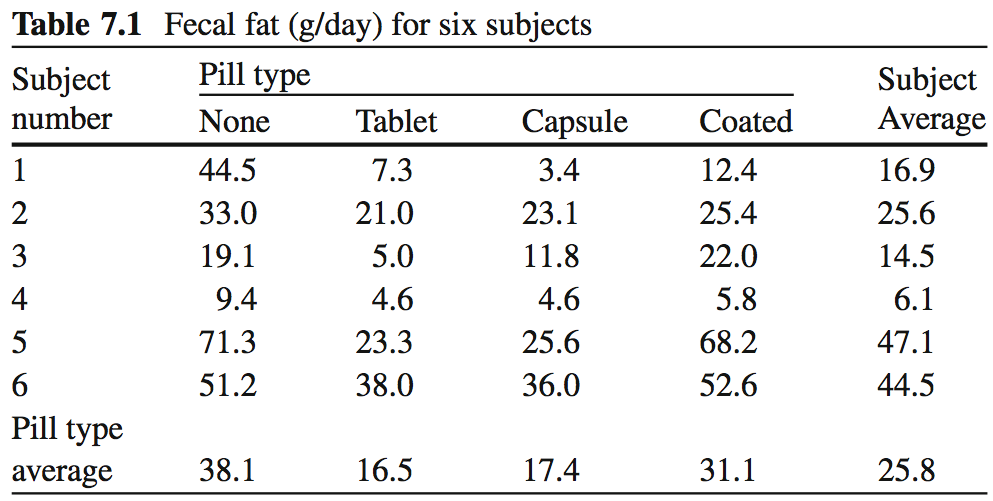
\includegraphics{VittinghoffTable71.png}
\caption{Fecal Fat dataset}
\end{figure}

\end{frame}

\begin{frame}{Option 1: non-hierarchical analysis (wrong)}
\protect\hypertarget{option-1-non-hierarchical-analysis-wrong}{}

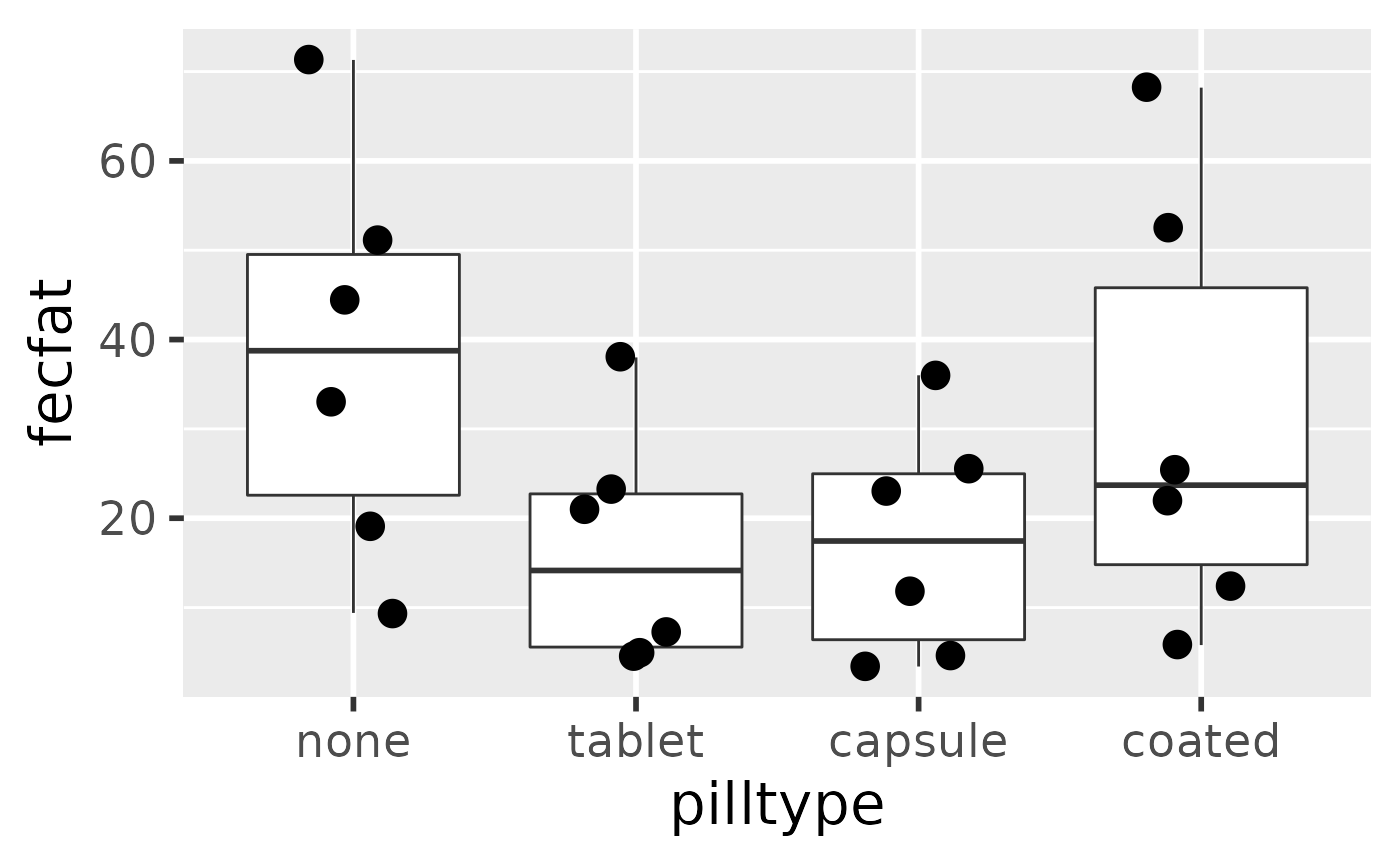
\includegraphics{../docs/articles/session_lecture_files/figure-beamer/boxplot-1.pdf}

\end{frame}

\begin{frame}[fragile]{Option 1: non-hierarchical analysis (wrong)}
\protect\hypertarget{option-1-non-hierarchical-analysis-wrong-1}{}

\footnotesize

\begin{Shaded}
\begin{Highlighting}[]
\NormalTok{fit1way <-}\StringTok{ }\KeywordTok{lm}\NormalTok{(fecfat }\OperatorTok{~}\StringTok{ }\NormalTok{pilltype, }\DataTypeTok{data=}\NormalTok{dat)}
\end{Highlighting}
\end{Shaded}

\begin{table}[ht]
\centering
\begin{tabular}{lrrrrr}
  \hline
 & Df & Sum Sq & Mean Sq & F value & Pr($>$F) \\ 
  \hline
pilltype & 3 & 2008.60 & 669.53 & 1.86 & 0.1687 \\ 
  Residuals & 20 & 7193.36 & 359.67 &  &  \\ 
   \hline
\end{tabular}
\caption{One-way analysis of variance table for fecal fat dataset} 
\end{table}

\begin{itemize}
\tightlist
\item
  Does not account for similarity of measurements within individual
\item
  Would be correct if each treatment were given to a different
  individual
\end{itemize}

\end{frame}

\begin{frame}{Option 2: 2-way AOV}
\protect\hypertarget{option-2-2-way-aov}{}

\begin{itemize}
\tightlist
\item
  Accounts for individual differences in mean fecal fat
\item
  Fits a coefficient for mean fecal fat per individual
\item
  Getting closer
\end{itemize}

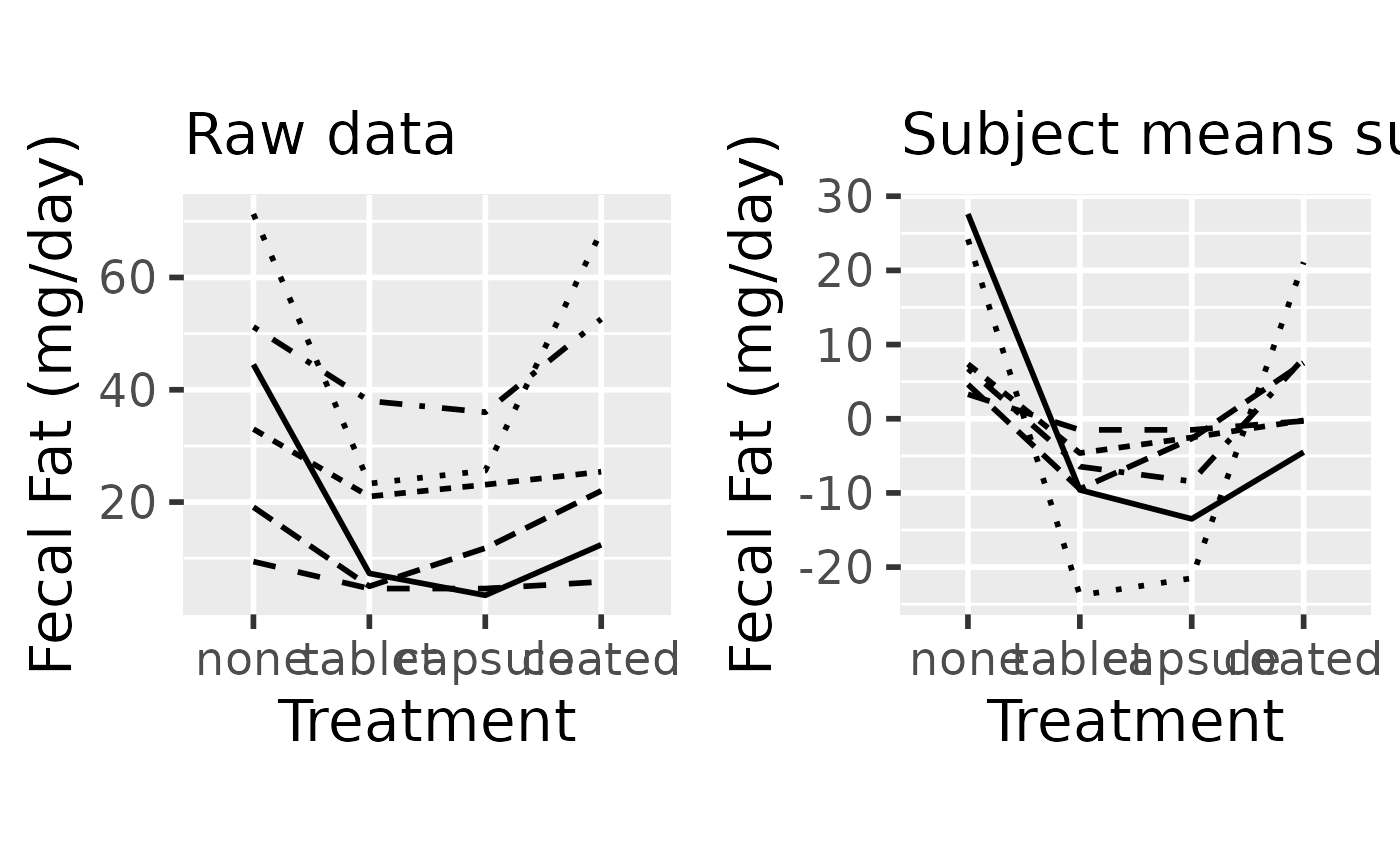
\includegraphics{../docs/articles/session_lecture_files/figure-beamer/ggspaghetti-1.pdf}

\end{frame}

\begin{frame}[fragile]{Option 2: 2-way AOV}
\protect\hypertarget{option-2-2-way-aov-1}{}

\footnotesize

\begin{Shaded}
\begin{Highlighting}[]
\NormalTok{fit1way <-}\StringTok{ }\KeywordTok{lm}\NormalTok{(fecfat }\OperatorTok{~}\StringTok{ }\NormalTok{pilltype, }\DataTypeTok{data=}\NormalTok{dat)}
\end{Highlighting}
\end{Shaded}

\begin{table}[ht]
\centering
\begin{tabular}{lrrrrr}
  \hline
 & Df & Sum Sq & Mean Sq & F value & Pr($>$F) \\ 
  \hline
pilltype & 3 & 2008.60 & 669.53 & 1.86 & 0.1687 \\ 
  Residuals & 20 & 7193.36 & 359.67 &  &  \\ 
   \hline
\end{tabular}
\caption{One-way analysis of variance table for fecal fat dataset} 
\end{table}

\begin{Shaded}
\begin{Highlighting}[]
\NormalTok{fit2way <-}\StringTok{ }\KeywordTok{lm}\NormalTok{(fecfat }\OperatorTok{~}\StringTok{ }\NormalTok{subject }\OperatorTok{+}\StringTok{ }\NormalTok{pilltype, }\DataTypeTok{data=}\NormalTok{dat)}
\end{Highlighting}
\end{Shaded}

\begin{table}[ht]
\centering
\begin{tabular}{lrrrrr}
  \hline
 & Df & Sum Sq & Mean Sq & F value & Pr($>$F) \\ 
  \hline
subject & 5 & 5588.38 & 1117.68 & 10.45 & 0.0002 \\ 
  pilltype & 3 & 2008.60 & 669.53 & 6.26 & 0.0057 \\ 
  Residuals & 15 & 1604.98 & 107.00 &  &  \\ 
   \hline
\end{tabular}
\caption{Two-way analysis of variance table. Note the similarity of the pilltype row.} 
\label{2}
\end{table}

\end{frame}

\begin{frame}{What happened??}
\protect\hypertarget{what-happened}{}

\begin{itemize}
\tightlist
\item
  1-way ANOVA correctly estimates the effect of pill type
\item
  However, 1-way ANOVA fails to accommodate the correlation within
  subjects
\item
  1-way ANOVA over-estimates the residual variance

  \begin{itemize}
  \tightlist
  \item
    under-estimates the significance of pill type
  \end{itemize}
\end{itemize}

\end{frame}

\begin{frame}{Regression models for 1 and 2-way ANOVA}
\protect\hypertarget{regression-models-for-1-and-2-way-anova}{}

\begin{itemize}
\tightlist
\item
  Recall for ordinary multiple linear regression: \begin{equation*}
  E[y|x] = \beta_0 + \beta_1 x_1 + \beta_2 x_2 + ... + \beta_p x_p
  \end{equation*}

  \begin{itemize}
  \tightlist
  \item
    \(x_p\) are the predictors or independent variables
  \item
    \(y\) is the outcome, response, or dependent variable
  \item
    \(E[y|x]\) is the expected value of \(y\) given \(x\)
  \item
    \(\beta_p\) are the regression coefficients
  \end{itemize}
\end{itemize}

\end{frame}

\begin{frame}{Regression models for 1 and 2-way ANOVA}
\protect\hypertarget{regression-models-for-1-and-2-way-anova-1}{}

\begin{itemize}
\item
  One-way ANOVA (person \(i\) with pill type \(j\)): \begin{equation*}
  \begin{aligned}
  FECFAT_{ij} &= \textrm{fecal fat measurement for person i with pill type j} \\
            &= \mu + PILLTYPE_j + \epsilon_{ij}
  \end{aligned}
  \end{equation*}
\item
  Two-way ANOVA: \begin{equation*}
  FECFAT_{ij} = \mu + SUBJECT_i + PILLTYPE_j + \epsilon_{ij}
  \phantom{\hspace{3cm}}
  \end{equation*}
\end{itemize}

Assumption:
\(\epsilon_{ij} \stackrel{iid}{\sim} N(0, \sigma_\epsilon^2)\)

\end{frame}

\hypertarget{correlations-within-subjects-icc}{%
\section{Correlations within subjects
(ICC)}\label{correlations-within-subjects-icc}}

\begin{frame}{Correlations within subjects}
\protect\hypertarget{correlations-within-subjects}{}

\begin{itemize}
\tightlist
\item
  One-way ANOVA fails because it does not account for the correlation of
  measurements within-person
\item
  How highly correlated are measurements on the same person? Consider
  subject \(i\), pill types \(j\) and \(k\):
\end{itemize}

\begin{equation*}
corr(FECFAT_{ij}, FECFAT_{ik}) = 
          \frac{cov(FECFAT_{ij}, FECFAT_{ik})}
               {sd(FECFAT_{ij}) sd(FECFAT_{ik})}
\end{equation*} * This is a measure of how large the subject effect is,
in relation to the error term

\end{frame}

\begin{frame}{Correlation within subjects}
\protect\hypertarget{correlation-within-subjects}{}

\begin{equation*}
\begin{aligned}
cov(FECFAT_{ij}, FECFAT_{ik}) &= cov(SUBJECT_i, SUBJECT_i) \\
                              &= var(SUBJECT_i) \\
                              &= \sigma_{subject}^2. \textrm{(definition)}
\end{aligned}
\end{equation*}

\begin{itemize}
\tightlist
\item
  Equality 1:

  \begin{itemize}
  \tightlist
  \item
    \(\mu\) and \(pilltype\) terms are assumed to be constant, so do not
    enter into covariance calculation
  \item
    residuals \(\epsilon\) are assumed to be independent
  \end{itemize}
\item
  Equality 2:

  \begin{itemize}
  \tightlist
  \item
    covariance with self is variance
  \end{itemize}
\end{itemize}

Recall \(SUBJECT_i\) is the term for individual in 2-way AOV. Now
\(\beta_i * subjectID\), will later be treated as a \textbf{random
variable}

\end{frame}

\begin{frame}{Correlation within subjects}
\protect\hypertarget{correlation-within-subjects-1}{}

Previous slide calculated \emph{covariance} for numerator of
correlation. Now calculate \emph{variance} for the denominator
(\({sd(FECFAT_{ij}) * sd(FECFAT_{ik})} = var(FECFAT_{ij})\))

\begin{equation*}
\begin{aligned}
var(FECFAT_{ij}) &= var(SUBJECT_i, SUBJECT_i) + var(\epsilon_{ij}) \\
                              &= \sigma_{subject}^2 + \sigma_{\epsilon}^2. \textrm{(definition)}
\end{aligned}
\end{equation*}

\begin{itemize}
\tightlist
\item
  Difference is that the independent residuals do contribute to
  \(var(FECFAT_{ij})\)
\item
  Variance is broken into componenets due to \emph{subject} and
  \emph{residual} variance
\end{itemize}

\end{frame}

\begin{frame}{Intraclass Correlation}
\protect\hypertarget{intraclass-correlation}{}

The correlation between two treatments \(j\) and \(k\) across subjects
\(i\) is: \begin{equation*}
\begin{aligned}
corr(FECFAT_{ij}, FECFAT_{ik}) & = 
          \frac{cov(FECFAT_{ij}, FECFAT_{ik})}
               {sd(FECFAT_{ij}) sd(FECFAT_{ik})} \\
      & = \frac{\sigma_{subj}^2}{\sigma_{subj}^2 + \sigma_{\epsilon}^2} \\
ICC & = \frac{\tau_{00}^2}{\tau_{00}^2 + \sigma_\epsilon^2}
\end{aligned}
\end{equation*}

\end{frame}

\begin{frame}{Intuition behind correlations within subjects}
\protect\hypertarget{intuition-behind-correlations-within-subjects}{}

\begin{figure}
\centering
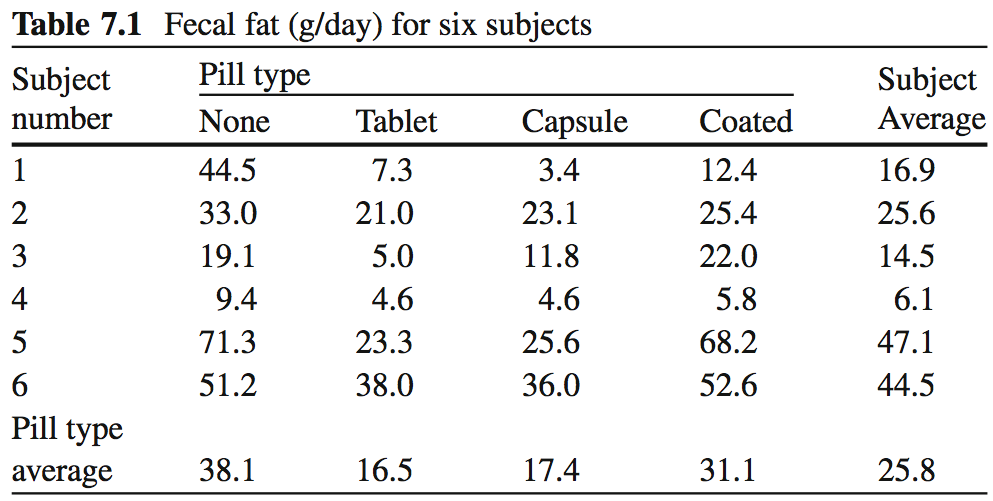
\includegraphics{VittinghoffTable71.png}
\caption{Fecal Fat dataset}
\end{figure}

\footnotesize

Variance of the subject averages (279.4) is increased by correlation of
measurements within individual.

\end{frame}

\begin{frame}[fragile]{Calculation of correlations within subjects
(ICC)}
\protect\hypertarget{calculation-of-correlations-within-subjects-icc}{}

What is your estimate of the variability due to subjects, from the 2-way
ANOVA? \footnotesize

\begin{Shaded}
\begin{Highlighting}[]
\KeywordTok{sum}\NormalTok{(}\KeywordTok{residuals}\NormalTok{(fit2way)}\OperatorTok{^}\DecValTok{2}\NormalTok{) }\OperatorTok{/}\StringTok{ }\DecValTok{15} \OperatorTok{/}\StringTok{ }\DecValTok{4} \CommentTok{#df=15, divided by 4 pilltypes}
\end{Highlighting}
\end{Shaded}

\begin{verbatim}
## [1] 26.74972
\end{verbatim}

\begin{Shaded}
\begin{Highlighting}[]
\FloatTok{279.419} \OperatorTok{-}\StringTok{ }\FloatTok{26.75} \CommentTok{#var(SUBJECT_i)}
\end{Highlighting}
\end{Shaded}

\begin{verbatim}
## [1] 252.669
\end{verbatim}

Residual variance is:

\begin{Shaded}
\begin{Highlighting}[]
\KeywordTok{sum}\NormalTok{(}\KeywordTok{residuals}\NormalTok{(fit2way)}\OperatorTok{^}\DecValTok{2}\NormalTok{) }\OperatorTok{/}\StringTok{ }\DecValTok{15} \CommentTok{#df=15}
\end{Highlighting}
\end{Shaded}

\begin{verbatim}
## [1] 106.9989
\end{verbatim}

\end{frame}

\begin{frame}{Calculation of correlations within subjects (ICC)}
\protect\hypertarget{calculation-of-correlations-within-subjects-icc-1}{}

Finally calculate ICC:

\begin{equation*}
\begin{aligned}
ICC &= \frac{\sigma_{subj}^2}{\sigma_{subj}^2 + \sigma_{\epsilon}^2} \\
    &= \frac{253}{253 + 107}
    &= 0.70
\end{aligned}
\end{equation*}

This calculation will become easier when we learn to estimate
\emph{random coefficients} in directly in the regression model.

\end{frame}

\hypertarget{random-and-fixed-effects}{%
\section{Random and fixed effects}\label{random-and-fixed-effects}}

\begin{frame}{The next step: a mixed effects model}
\protect\hypertarget{the-next-step-a-mixed-effects-model}{}

\begin{itemize}
\item
  Two-way ANOVA is a fixed effects model: \[
  FECFAT_{ij} = \beta_0 + \beta_{subject i} SUBJECT_i + \beta_{pilltype j} PILLTYPE_j + \epsilon_{ij}
  \]

  \begin{itemize}
  \tightlist
  \item
    Assumption:
    \(\epsilon_i \stackrel{iid}{\sim} N(0, \sigma_\epsilon^2)\)
  \end{itemize}
\item
  Instead of fitting a \(\beta_{subject i}\) to each individual, assume
  that subject effects are selected from a distribution of possible
  subject effects: \[
  FECFAT_{ij} = \mu + SUBJECT_i + \beta_{pilltype j} PILLTYPE_j + \epsilon_{ij}
  \] where \(SUBJECT_i \stackrel{iid}{\sim} N(0, \sigma_{subj}^2)\)
\item
  Here subject is a \emph{random} effect, and pill type is a
  \emph{fixed} effect.
\item
  This is also a random intercept model
\end{itemize}

\end{frame}

\begin{frame}{Random and fixed effects}
\protect\hypertarget{random-and-fixed-effects-1}{}

\begin{figure}
\centering
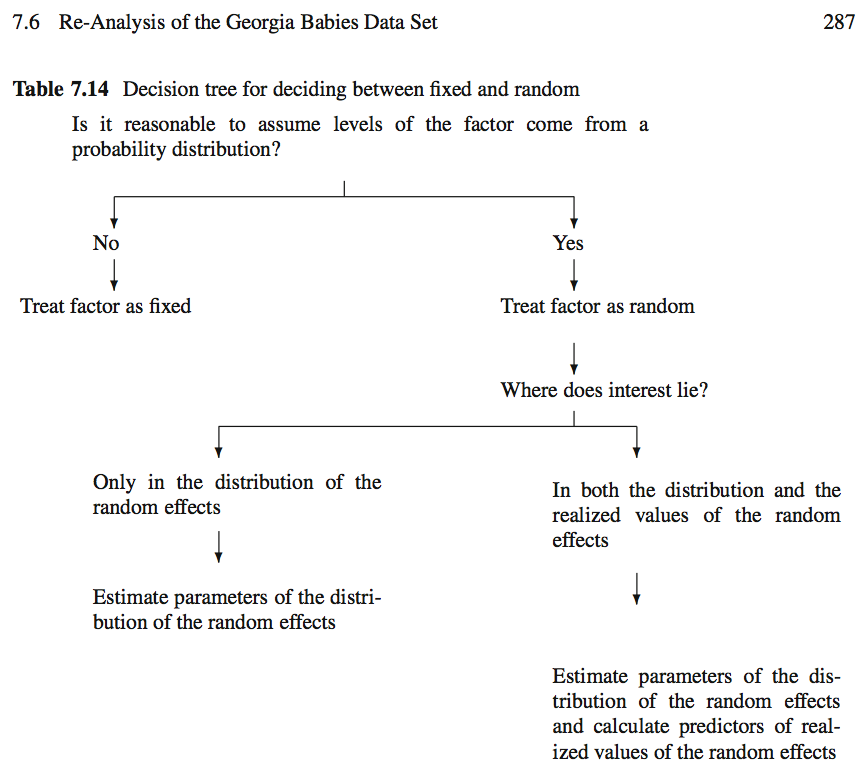
\includegraphics{VittinghoffTable714.png}
\caption{Random and Fixed Effects}
\end{figure}

\end{frame}

\begin{frame}{Summary: correlations within subjects}
\protect\hypertarget{summary-correlations-within-subjects}{}

\begin{itemize}
\tightlist
\item
  Subject-to-subject variability simultaneously raises or lowers all the
  observations on a subject

  \begin{itemize}
  \tightlist
  \item
    induces correlation of within-subject measurements
  \end{itemize}
\item
  Variability of individual measurements can be separated into that due
  to subjects and that left to residual variance.

  \begin{itemize}
  \tightlist
  \item
    \(var(FECFAT_{ij}) = \sigma_{subj}^2 + \sigma_{\epsilon}^2\)
  \end{itemize}
\item
  2-way ANOVA does not directly estimate variability due to subjects

  \begin{itemize}
  \tightlist
  \item
    variance of coefficients for individual is not too far off
  \end{itemize}
\end{itemize}

\end{frame}

\begin{frame}{Summary: hierarchical data}
\protect\hypertarget{summary-hierarchical-data}{}

\begin{itemize}
\tightlist
\item
  Estimates of coefficients (or ``effect sizes'') are unchanged by
  hierarchical modeling
\item
  Ignoring within-subject correlations results in incorrect estimates of
  variance, F statistics, p-values

  \begin{itemize}
  \tightlist
  \item
    not always ``conservative''
  \end{itemize}
\item
  Intraclass Correlation (ICC) provides a measure of correlation induced
  by grouping
\item
  Should be able to recognize fixed and random effects
\end{itemize}

\end{frame}

\end{document}
